\chapter*[Introdução]{Introdução}
\addcontentsline{toc}{chapter}{Introdução}

% Este documento apresenta considerações gerais e preliminares relacionadas 
% à redação de relatórios de Projeto de Graduação da Faculdade UnB Gama 
% (FGA). São abordados os diferentes aspectos sobre a estrutura do trabalho, 
% uso de programas de auxilio a edição, tiragem de cópias, encadernação, etc.

\section*{O uso de gerenciadores} % (fold)
\label{sec:o_uso_de_gerenciadores}

% section o_uso_de_gerenciadores (end)

Um dos processos  que novos usuários Linux tem dificuldade em se adaptar é a instalação de novas aplicações. Hoje é comum haver nas plataformas uma aplicação que centraliza a instalação das demais aplicações. Visto como uma loja em algumas plataformas, o gerenciador de aplicações tão comum nos dias atuais era, há alguns anos um diferencial dos sistemas Linux. Usuários do sistema operacional Windows que iniciavam o aprendizado do sistema Linux  tinham dificuldade para compreender que não precisavam acessar o site de um fabricante como a Adobe para instalar o leitor de PDF, ou frequentar sites como Baixaki para fazer o \textit{download} de aplicações diversas. Tudo o que precisavam era abrir o terminal e com alguns comandos o software era instalado de uma fonte confiável. 

A compreensão deste processo abria novas fronteiras para o  usuário, que agora buscava expandir seu conhecimento e testar novas aplicações dentre as milhares que estavam à sua disposição. Obviamente que o processo de instalação e remoção de pacotes eventualmente torna-se dependente de uma ferramenta que possibilite realizar buscas por aplicações e filtragem das aplicações retornadas. E este é o ponto onde os novos usuários encontravam maiores dificuldades. 

\subsection*{As primeiras dificuldades} % (fold)
\label{sub:as_primeiras_dificuldades}

% subsection as_primeiras_dificuldades (end)

Quando realizadas em linha de comando, as buscas por pacotes podem ser complexas para usuários inexperientes em relação ao uso de comandos no terminal, e a ordenação dos resultados é ainda menos intuitiva. Uma busca por \textit{``pdf''} no {\code apt} leva hoje a um resultado que, além de estourar o \textit{buffer} de linhas da janela do terminal, apresenta o popular {\code evince} aproximadamente como $14ª$ opção dentre os  pacotes disponíveis para instalação, como por ser observado na \autoref{fig:figuras_search_pdf}, dependendo das listas de repositórios adicionados na distribuição e qual gerenciador esta sendo usado.

\begin{figure}[h]
  \centering
	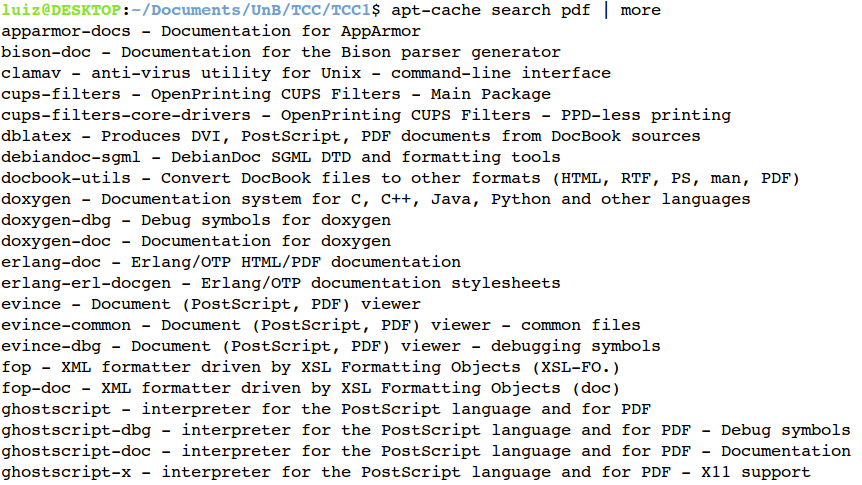
\includegraphics[width=0.72\textwidth]{figuras/search_pdf}
  \caption{Apresentação de resultados da busca do termo \textit{pdf} usando o {\code apt-cache}}
  \label{fig:figuras_search_pdf}
\end{figure}

Alem disso, aplicações que não tem relação com leitores de \textit{pdf}, tais como o antivírus {\code clamav} ou o produtor de documentação {\code doxygen}, aparecem antes do {\code evince} devido às regras de ordenação do APT. O primeiro parâmetro de ordenação do APT é o repositório em que o pacote esta localizado. Essa ordem é definida de acordo com os dados inseridos no {\code /etc/apt/sources.list} e {\code /etc/apt/sources.list.d}.  ordenação alfabética dos repositórios e por terem, seja em seu nome, descrição ou \textit{tags}, a sequência \textit{``pdf''}. Por fim, os pacotes selecionados em um mesmo repositório serão ordenados alfabeticamente.

O resultado é ainda menos preciso quando utilizada a interface do {\code apt} ao invés do {\code apt-cache}. Como esta interface apresenta todos os resultados em uma única ordenação alfabética, temos na $11ª$ posição um visualizador de PDF (\textit{apvlv}), porém o popular {\code evince} nem mesmo entra na lista dos 20 primeiros.

\begin{figure}[h]
  \centering
	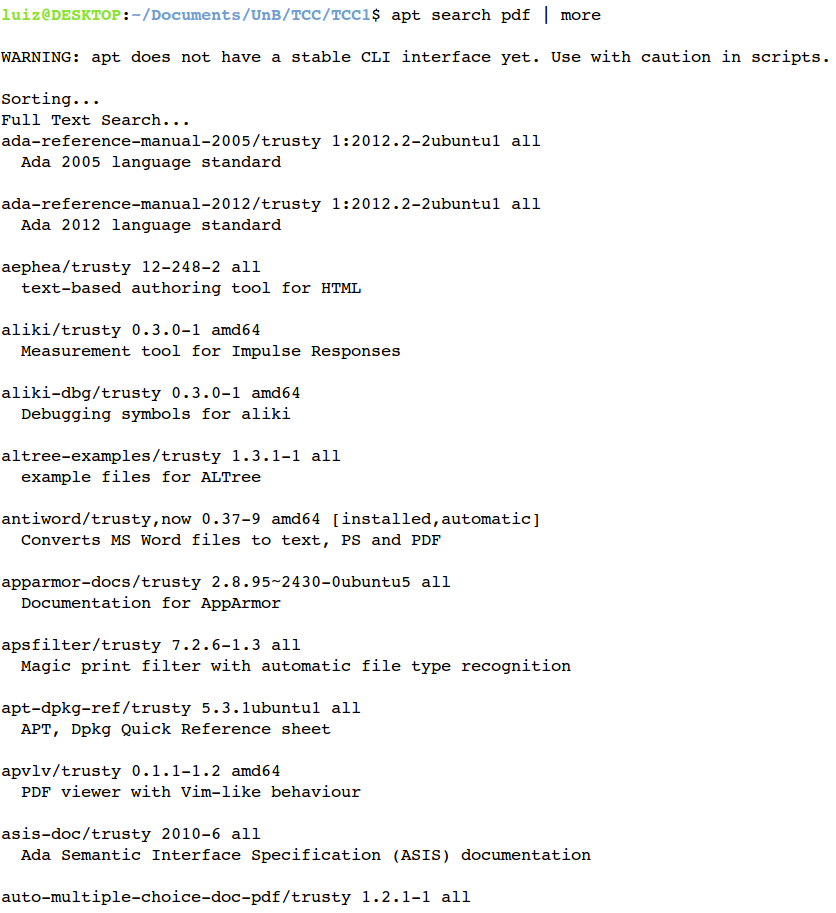
\includegraphics[width=0.72\textwidth]{figuras/search_pdf_ii}
  \caption{Apresentação de resultados da busca do termo \textit{pdf} usando o {\code apt}}
  \label{fig:figuras_search_pdf_ii}
\end{figure}


Dentre os diversos gerenciadores de repositório utilizados atualmente para a instalação de pacotes em distribuições Linux, podemos apontar alguns que se destacam por virem instalados de padrão nas distribuições mais comuns hoje e, consequentemente sendo os mais  utilizados, como o {\code apt} ou o {\code yum}.

Porém, os principais gerenciadores possuem em comum o mesmo problema de ordenação dos resultados de uma busca. A apresentação de resultados de uma busca não é personalizável, não permitindo classificar a listagem de pacotes por nome, por exemplo, nem fazem \textit{matching} de aproximação  entre o pacote pesquisado e os possíveis candidatos. Desta forma a procura por um pacote do qual não se tenha o nome correto pode se tornar cansativa e desgastante, especialmente para um novo usuário Linux, que desconhece de ferramentas como o {\code grep, more} ou {\code  less}. 


% Nesto documento serão apresentados os \lnameref{cha:objetivos} que deseja-se alcançar com este trabalho. Em seguida será apresentada a \lnameref{cha:fundamentacao} levantada para a produção do estudo. Apresentada a fundamentação, seguirá uma \lnameref{cha:delimitacao}, afim de restringir as propostas do trabalho e estabelecer oportunidades para trabalhos posteriores. Em seguida será apresentada a \lnameref{cha:metodologia} adotada no trabalho para que fossem alcançados os \lnameref{cha:resultados} apresentados no último capítulo.